% お使いの環境に合わせて以下3行のdocumentclassをお選びください。
\documentclass[twocolumn]{jarticle} % pLaTeX
%\documentclass[uplatex,twocolumn]{jsarticle}  % upLaTeX
%\documentclass[xelatex,twocolumn,ja=standard,enablefam=true]{bxjsarticle} % XeLaTeX

\usepackage{rsj2024j}
\usepackage[dvipdfmx]{graphicx}
\usepackage{url}
\usepackage{tikz}

\begin{document}
\title{第42回日本ロボット学会学術講演会 原稿の書き方}
\author{〇著者甲姓\ 著者甲名(著者甲所属)\ \ 著者乙姓\ 著者乙名(著者乙所属)}
\abstract{From 2023, authors are encouraged to write an article's abstract in either Japanese or English. Ab-stracts should be 3-6 lines long (100 words or less in English). If authors use simultaneous submission of the [Letter], an abstract in English is required. If authors are not using simultaneous submission and will submit the article in English to other journals in the future, an abstract in English is not recommended due to the risk of being considered self-plagiarism. }
\setlength{\baselineskip}{4.4mm}	% 行間の設定
\maketitle
\thispagestyle{empty}
\pagestyle{empty}

\section{講演論文原稿作成方法について}
講演論文原稿(PDF形式のみ)の投稿はインターネット経由で行います.
詳細は,第42回日本ロボット学会学術講演会のウェブサイト\cite{website}をご参照ください.原稿は以下の要領で作成してください.

\begin{enumerate}
    \item {\bfseries Microsoft Word の場合}\\
    ウェブサイト\cite{website}から\verb|sample2024j.doc|をダウンロードして講演論文原稿を作成してください.
    MS WordやOSのバージョンによってはレイアウトが崩れる場合があります.
    そうした場合は,適宜\verb|sample2024j.pdf|の書式に合うように原稿を作成してください.

  \item {\bfseries \TeX (pLaTeX/upLaTeX/XeLaTeX) の場合}\\
    ウェブサイト\cite{website}から\verb|sample2024j_tex.zip|をダウンロードし,その中に含まれる\verb|sample2024j.tex| と \verb|rsj2024j.sty|をお使いください.ダウンロードしたものはpLaTeXでコンパイルできる状態になっています.upLaTeXあるいはXeLaTeXをお使いの方は\verb|sample2024j.tex|の先頭部分のコメントアウトされた\verb|documentclass|コマンドをお使いください.
    なお,\TeX では,\verb|sample2024j.pdf|の書式と一部異なる部分があります.ご了承ください.
  \item {\bfseries Typst の場合}\\
    Typst\cite{typst} は\TeX{}に似た新しい組版システムです.RSJ2024ではTypstのテンプレートもご用意いたしました.ウェブサイト\cite{website}から\verb|sample2024j_typst.zip|をダウンロードし,その中に含まれる\verb|sample2024tj.typ|,\verb|samplebib.bib|(参考文献ファイル)および\verb|rsj2024t.typ|(\TeX{}のスタイルファイルのような役割のファイル)をお使いください.
    なお,Typstでは\verb|sample2024j.pdf|の書式と一部異なる部分があります.ご了承ください.
    \item {\bfseries その他の場合}\\        
    \verb|sample2024j.pdf|の書式に合うように原稿を作成してください.
\end{enumerate}

作成したファイル(dviファイル,Wordファイル等)からPDFファイルを作成してください.
このときの画質,セキュリティ,余白等について注意してください.詳細は,ウェブサイト\cite{website}をご参照ください.
また,作成されたPDFファイルを Adobe Acrobat Readerで開いてご確認ください.
確認事項については,ウェブサイト\cite{website}をご参照ください.

\section{講演論文原稿書式について}
\subsection{原稿枚数について}
講演論文原稿は1ページ以上4ページ以内です.
ファイルの容量は3Mバイト(論文参考用動画ファイルを併せてご投稿される場合は,動画ファイルを含めて4Mバイト)までです.
規定ページを超えるものは掲載いたしません.また,容量制限を超えるものは投稿できません.

\subsection{和文原稿の場合}
\subsubsection{原稿の体裁}
A4版白紙に縦250mm,横170mmの枠内に収まるようにお願いします(余白は上側20mm,下側27mm,左右20mm).
本文は10ポイント程度をご使用ください.
提出された講演論文原稿は,そのまま予稿集に掲載します.
原稿の書き方が不適当にならないようにご留意ください.
詳細については,ウェブサイト\cite{website}をご参照ください.

\subsubsection{図と表について}
図の例を図\ref{fig:sample}に示します.講演論文原稿はPDFファイルとなりますので,図・表はカラーで作成していただいても構いません.
ただし,印刷しても問題ない程度の解像度を持ち,
かつアップロードの際のファイルサイズ上限を越えない大きさとなるようにご留意ください.

%図の入れ方
\begin{figure}[tb]
  \centering
  \large
  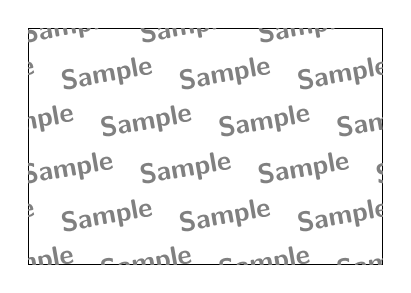
\begin{tikzpicture}
    \draw rectangle++(4.5,3);
    \clip rectangle++(4.5,3);
    \foreach\x in{0,1,2,3,4}{
      \foreach\y in{0,1,2,3,4,5,6}{
        \path(\x*1.5-\y*0.5,\y*0.6)node[rotate=10,text=gray]{\sffamily\bfseries\itshape Sample };
      }
    }
  \end{tikzpicture}
  % eps 画像を貼る場合は includegraphics をお使いください。
  % \includegraphics[width=45mm]{samplefig2.eps}
  \caption{サンプル画像}
  \label{fig:sample}
\end{figure}

\subsubsection{参考文献}
文献の引用は本文中に\cite{website}\cite{yamada2000}のように通し番号を付して書き(上付にはしない),参考文献を本文の最後にまとめて書いてください.
参考文献の書式は,日本ロボット学会誌の執筆要項\cite{rsj_rules}に準拠してください.

\subsection{和文原稿の場合の注意点}
学術講演会の和文原稿には,和文題名,和文著者名を掲載してください.
英文題目,英文著者名は併記しないでください.
図中のキャプションや図名も和文とします.

ただし,レター同時投稿オプションを利用する場合は,レター原稿のフォーマットにしたがって和文・英文題目,和文・英文著者名を併記しても構いません.
レター原稿中の図名及び説明文が英語記載となっているため,講演会和文原稿の図名及び説明文も英語で記載しても構いません.

また,2023年より,和文または英文要旨(選択可)の掲載を推奨(レター同時投稿オプションを利用する場合は必須)としています.
要旨は3\textasciitilde6行程度(英文の場合,100語以内)とします.
和文,英文原稿ともキーワードの掲載は必用ありません.

\subsection{英文原稿の場合}
英文原稿の執筆要綱は和文原稿のそれに準じます.
英文による題目,著者名をご記入下さい.
和文による題目,著者名等は不要です.
また,英文で,要旨,本文,図中のキャプションや図名もご記入ください.

\section{講演申し込みおよび電子入稿}
2019 年より講演申し込みと電子入稿の締め切りが異なるものとなり,2 段階での手続きとなりました.
講演申込締切までに,講演題目・著者名・講演概要などを登録し,講演の申し込みをしてください.
その後,論文投稿〆切日までに,講演論文原稿ファイル(PDF 形式)をアップロードしてください.
詳細については,ウェブサイト\cite{website}をご参照ください.

%% 謝辞(必要な場合のみ)
%%\begin{acknowledgements}
%%\end{acknowledgements}

\section{レター同時投稿について}
2020年より,日本ロボット学会学術講演会から日本ロボット学会誌へのレター同時投稿を受け付けています.
日本ロボット学会学術講演会に投稿した講演論文を「そのまま」の内容(フォーマットは異なります)でレター(速報性を有する研究報告.最大 4 ページ)に投稿することが可能ですので,これを同時に受け付けます. 

レター原稿の作成と投稿に関する詳細については,日本ロボット学会誌の規定[3]をご覧頂ければと思いますが,講演会の論文投稿と同時に,ロボット学会ウェブサイトに掲載の論文投稿システムより同内容をレターフォーマットで投稿して頂ければ,査読プロセス(速報性を重視するため初回査読期間は 15 日以内)を経て Acceptされた論文が,講演会後に順次オンラインに掲載されます.

学術講演会等の講演論文を論文誌に投稿する際には「新たな内容の追加や内容の充実が必要である」としていますが,日本ロボット学会が主催する学術講演会については,この規定の対象外としているため,レター同時投稿が可能となっています.
この機会を使って,是非,レター投稿をご検討下さい.

なお,レターは最大4ページですが,4ページ未満の原稿も受け付けます.レター同時投稿の原稿作成ならびに投稿については,ウェブサイト\cite{website}をご参照ください.


%% 謝辞(必要な場合のみ)
%\begin{acknowledgements}
%    Thanks.
%\end{acknowledgements}

\small
\begin{thebibliography}{9}
%%%%%%%%%%%%%%%%%%%%%%%%%%%%%%%%%%%%%%%%%%%%%%%%%%%%%%%%%%%%%%%%%%%%%%%%%%%%%%%

\bibitem{website}
``第42回日本ロボット学会学術講演会のウェブサイト'',
  \url{https://ac.rsj-web.org/2024/}
\bibitem{typst}
  ``Typst website'',
  \url{https://typst.app}
\bibitem{yamada2000}
  山田太郎,鈴木一郎:
  ``第100回日本ロボット学会講演会用原稿の書き方'',
  日本ロボット学会誌, vol. 99, no. 4, pp. 8--12, 2082.
\bibitem{rsj_rules}
  ``日本ロボット学会誌・寄稿および査読に関する規則集'',
  \url{https://www.rsj.or.jp/content/files/data_rules/F-02.pdf}
%%%%%%%%%%%%%%%%%%%%%%%%%%%%%%%%%%%%%%%%%%%%%%%%%%%%%%%%%%%%%%%%%%%%%%%%%%%%%%%
\end{thebibliography}

\end{document}
